\begin{figure}
\begin{center}
    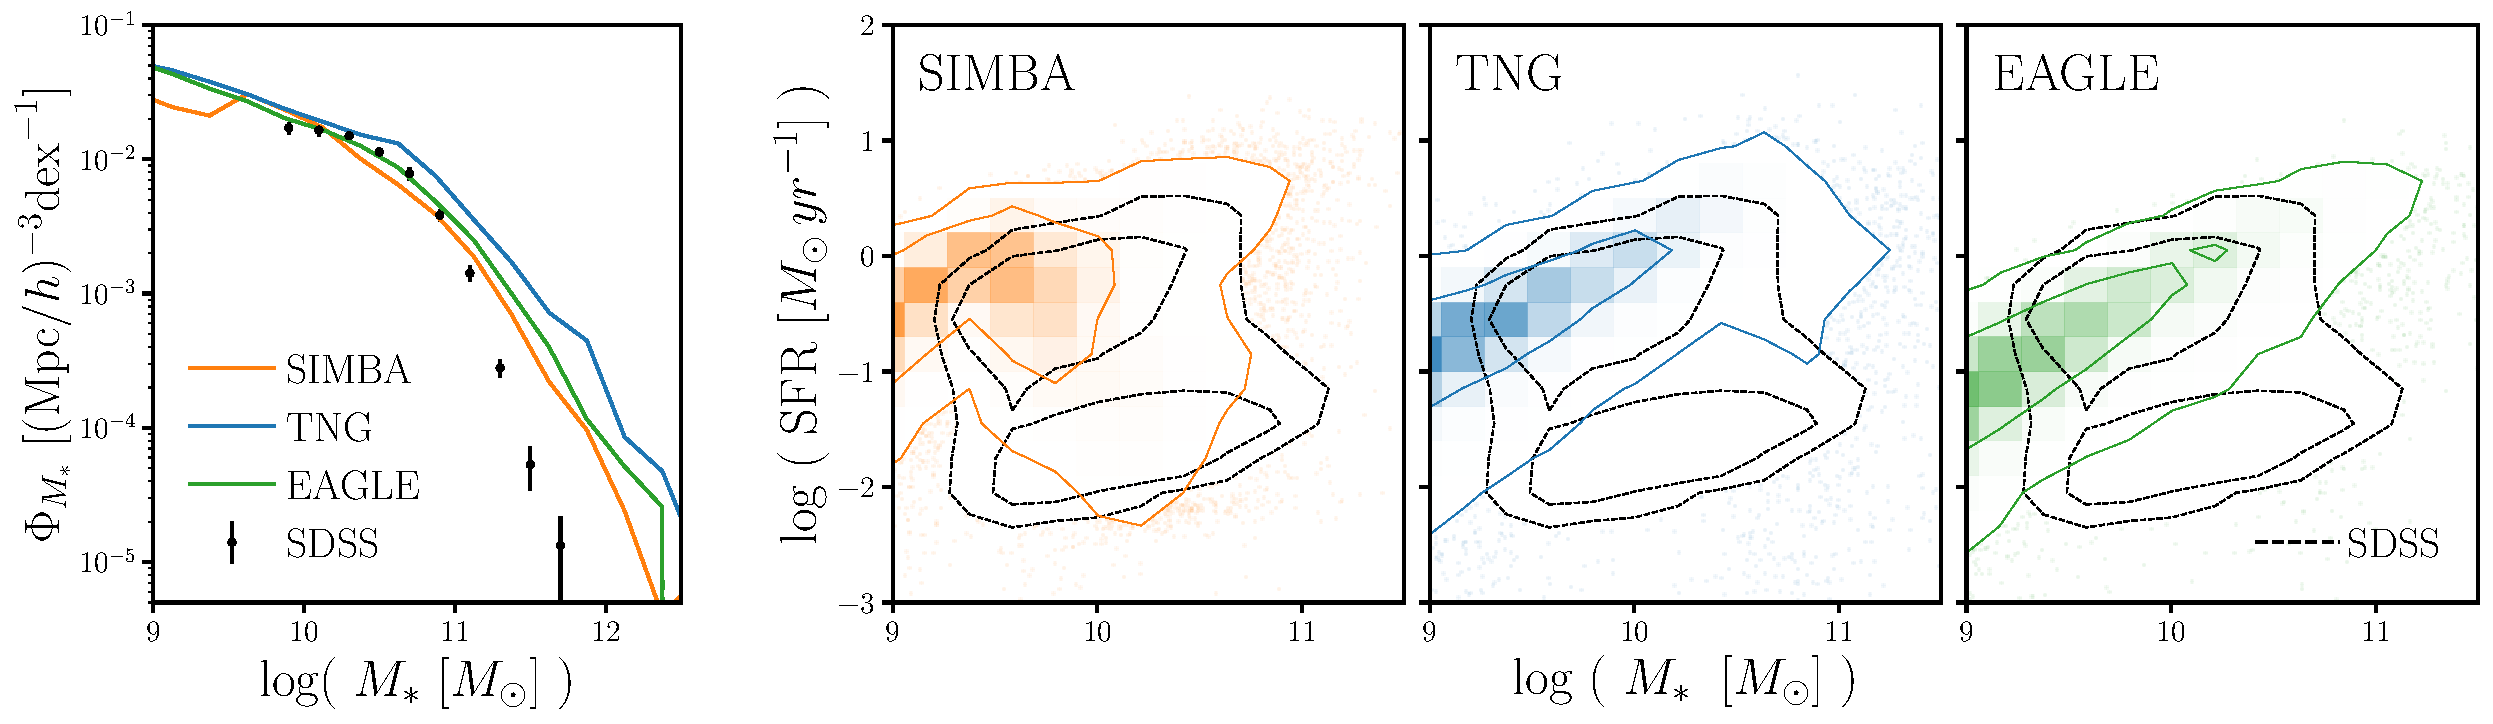
\includegraphics[width=\textwidth]{figs/smf_m_sfr.pdf}
    \caption{\label{fig:smf_msfr}
    The stellar mass functions, $\Phi_{M_*}$ (left-most panel), and $M_*-\sfr$
    relation (right panels) of galaxies in three cosmological hydrodynamic 
    simulations: SIMBA (orange), TNG (blue), and EAGLE (green). 
    For reference, we include $\Phi_{M_*}$ (black) and the $M_*-\sfr$ relation 
    (black dashed) of from SDSS observations. Uncertainties for the 
    SDSS $\Phi_{M_*}$ are derived using jackknife resampling. We describe the
    simulations and observations in Section~\ref{sec:sims}. 
    There are significant differences between the $M_*-\sfr$ relations of
    SDSS and the simulations, which are driven by the inconsistencies
    between the simulations' theoretical $M_*$ and $\sfr$ predictions
    and the SDSS measurements.
    A forward modeling approach, where we construct synthetic observations
    for the simulations, reduces the inconsistencies and enables an
    apples-to-apples comparison between simulations and observation. 
    \emph{Furthermore, differences
    in $\Phi_{M_*}$ and the $M_*-\sfr$ relations among the hydrodynamic simulations 
    highlight how they predict galaxy populations with significantly different
    physical properties.} 
    }
\end{center}
\end{figure}

\section{Data}\label{sec:sims}
In this paper, we present the Empirical Dust Attenuation (\eda) model and
demonstrate how it can be used in a forward modeling approach to compare galaxy
populations in simulations and observations. For our simulations, we use three large-scale
cosmological hydrodynamical simulations: the IllustrisTNG (hereafter TNG),
EAGLE, and SIMBA. For our observations, we use a galaxy sample derived from
SDSS. Below, we briefly describe the hydrodynamical simulations and the SDSS
observations used throughout this work.

In Figure~\ref{fig:smf_msfr}, we present the stellar mass functions,
$\Phi_{M_*}$ left-most panel, and $M_*-\sfr$ relations (right panels) of
galaxies in the  SIMBA (orange), TNG (blue), and EAGLE (green) cosmological
hydrodynamic simulations.  For reference, we include $\Phi_{M_*}$ and the 
$M_*-\sfr$ relation for SDSS observations. For the simulations, $M_*$ is the
total stellar mass within the subhalo and $\sfr$ is the instantaneous $\sfr$ in the
dense and cold star-forming gas. 
We do not impose any selection cuts on the simulations in
Figure~\ref{fig:smf_msfr} and include both central and satellite galaxies. 
For SDSS, $M_*$ is estimated using $\mathtt{kcorrect}$~\citep{blanton2007a} 
assuming a~\cite{chabrier2003} initial mass function and $\sfr$ is from the
current release of \cite{brinchmann2004}\footnote{\url{http://www.mpa-garching.mpg.de/SDSS/DR7/}}.
The uncertainties for the SDSS SMF are derived from jackknife resampling.
We find striking differences between the $M_*-\sfr$ relation of SDSS and
the simulations, which underscore the need for a forward modeling approach.
While the $M_*$ and $\sfr$ of simulations represent theoretical
predictions, the values for SDSS are subject to, for example, $\sfr$
measurement limits, inconsistencies among $\sfr$ tracers, and aperture
effects.
By constructing synthetic observations for the simulations with forward
models, the simulations can be more consistently compared to
observations~\citep[see \eg][Starkenburg et al. in prep.]{dickey2020}
Figure~\ref{fig:smf_msfr} also illustrates that the hydrodynamical simulations
predict different SMFs and $M_*-\sfr$ relations from each other.
This difference, which was also recently highlighted in \cite{hahn2019c},
demonstrates that \emph{the hydrodynamical simulations predict galaxy
populations with significantly different physical properties from one
another}.

\subsection{IllustrisTNG100} \label{sec:tng}
The IllustrisTNG100 simulation\footnote{\url{https://www.tng-project.org/}}
is a cosmological hydrodynamic simulation of comoving volume 
$(110.7\,\mpc)^3$, with a particle mass resolution of $7.6 \times 10^{6}\ M_\odot$ for dark matter and $1.4 \times 10^{6}\ M_\odot$ for baryonic particles~\citep{nelson2018, pillepich2018, springel2018}. It improves on
the original Illustris simulation\footnote{\url{http://www.illustris-project.org}}~(\citealt{vogelsberger2014, genel2014};
public data release by~\citealt{nelson2015}), by including
magneto-hydrodynamics and updated treatments for galactic winds, metal
enrichment, and AGN feedback. Most notably, TNG uses a new implementation for
feedback from SMBH, where feedback energy is injected in the form of a kinetic
AGN-driven wind at low SMBH accretion rates~\citep{weinberger2018}. This new
implementation has been shown to alleviate discrepancies found between the
original Illustris and observations for $> 10^{13-14} M_\odot$ massive halos. 
%TNG has a baryonic mass resolution of $1.4\times10^6M_{\sun}$ \ch{temporal resolution?}\tks{why would you need to know temporal resolution? for the SFH?}.
%\todo{details on the following properties that we use in the paper: SFH, ZH}

\subsection{EAGLE} \label{sec:eagle} 
The Virgo Consortium's EAGLE
project\footnote{\url{http://www.eaglesim.org}}~\citep{schaye2015, crain2015,
mcalpine2016} is a publicly available suite of cosmological hydrodynamic
simulations constructed using {\sc Anarchy} (Dalla Vecchia et al. in prep.; 
see also Appendix A of \citealt{schaye2015}), a modified version of the 
{\sc GADGET-3} code~\citep{springel2005}. We use the L0100Ref simulation,
which has a comoving volume of $(100\,\mpc)^3$, and a baryonic mass resolution of $1.81\times 10^6M_{\sun}$. %It 
%that includes a conservative pressure-entropy formulation for the smoothed particle hydrodynamics calculation, artificial viscosity, artificial conduction and the time limiter that improve hydrodynamic computation performance. 
EAGLE has subgrid models for star formation, stellar mass loss, metal enrichment
and stellar feedback that stochastically inject thermal energy in the ISM as
in~\citep{dallavecchia2012}. The feedback energy from AGN is also added to
surrounding gas stochastically~\citep{booth2009}. Parameters of the stellar 
feedback and SMBH accretion are calibrated to broadly reproduce the $z=0$ 
stellar mass function and galaxy stellar size-stellar mass relation. Meanwhile, 
the AGN feedback efficiency is calibrated to match the SMBH-galaxy mass relation. 
%\todo{details on the following properties that we use in the paper: SFH, ZH}

\subsection{SIMBA} \label{sec:simba}
The {\sc Simba} simulation suite~\citep{dave2019}, the successor to {\sc
Mufasa}~\citep{dave2016, dave2017, dave2017a}, is a cosmological hydrodynamical
simulation constructed using {\sc Gizmo}, a meshless finite mass hydrodynamics 
code~\citep{hopkins2015, hopkins2017}. Of the simulations, we use
`m100n1024', which has a box size of $(100\,h^{-1}\,\mpc)^3$ and baryonic 
mass resolution of $1.82 \times 10^7\ M_\odot$. The simulation uses the same
subgrid models as {\sc Mufasa} for $\rm H_2$ based star formation, decoupled
two-phase winds for star formation driven galactic winds, and feedback from 
Type I supernovae and AGB stars. {\sc Simba} uses a two-mode SMBH accretion 
model, torque-limited accretion for cold gas~\citep{angles-alcazar2017} and 
Bondi-based accretion for hot gas, and two-mode AGN feedback. %which ejects bipolar kinetic winds with $\sim 10^3 \kms$ for high SMBH accretion rate, and launches winds with increased velocity of $\sim 8000 \kms$ for low SMBH accretion of Eddington ratio below 2 \%.
%\todo{details on the following properties that we use in the paper: SFH, ZH}

\subsection{SDSS Galaxies} \label{sec:obs} 
For our observations, we use a galaxy sample derived from SDSS observations. 
We begin with the volume-limited \cite{tinker2011} sample derived from the SDSS
DR7~\citep{abazajian2009} NYU Value-Added Galaxy
Catalog~\citep[VAGC;][]{blanton2005},which has a $M_* > 10^{9.7} M_\odot$
completeness limit. 
We focus on observables that can be consistently defined and derived in both simulations 
and observations: the $r$-band absolute magnitude, $M_r$, the optical $\gr$
color, and the $\fnuv$ color. 
We use $FUV$, $NUV$, $r$ and $g$ band absolute magnitudes from the NASA-Sloan
Atlas\footnote{\url{http://nsatlas.org/}}, which is re-reduction of SDSS DR8
\citep{aihara2011} that includes an improved background subtraction~\citep{blanton2011} 
and near and far UV photometry from GALEX. These absolute magnitudes are
derived using $\mathtt{kcorrect}$~\citep{blanton2007a}, assuming
a~\cite{chabrier2003} initial mass function. 

We impose a $M_r < -20$ completeness limit on the \cite{tinker2011} sample.
\chedit{
    We also impose completeness limits in the $FUV$ and $NUV$ bands. 
    UV fluxes in the NASA-Sloan Atlas are measured using forced photometry on
    GALEX so galaxies can have $FUV$ and $NUV$ fluxes $\leq 0$. 
    First, we exclude these galaxies from the SDSS sample. 
    Furthermore, $\mathtt{kcorrect}$ UV absolute magnitudes are poorly
    constrained for galaxies with low UV fluxes. 
    We compare the reconstructed $FUV$ and $NUV$ fluxes from
    $\mathtt{kcorrect}$ to the measured fluxes and determine the flux limits
    below which the fluxes are in good agreement. 
    The flux limits correspond to completeness limits of $M_{FUV} < -13.5$  and
    $M_{NUV} < -14.0$, which we also impose on the SDSS sample. 
    In total, our SDSS sample has 4,451 galaxies.
}

\subsection{Forward Modeling Observations} \label{sec:fm} 
One of the main goals of this work is to conduct an ``apples-to-apples''
comparison between the simulations and observations. 
A crucial step in this comparison is to \emph{forward model} the
observables from the simulations. 
The simulations can then be directly compared to observations in
observational-space. 
This means that the comparison does not rely on measured galaxy properties,
which are impacted by variations, inconsistencies, and biases of different
methods~\citep{dickey2020}. 
The comparison can also include selection functions and observational systematic
effects through the forward model. 
In this work, we use $r$-band luminosity ($M_r$), optical color ($\gr$),
and UV color ($\fnuv$) as our observables. 

As the first step in our forward model, we construct SEDs for all
of the simulated galaxies based on their star formation and metallicity
histories (SFH and ZH) using the Flexible Stellar Population Synthesis
model~\citep[$\mathtt{FSPS}$;][]{conroy2009, conroy2010}. For each simulated
galaxy, we bin the total stellar mass formed by age ($t$) and metallicity
($Z$). We use a consistent $t$, $Z$ grid for all of the simulations
to account for the variable time and mass resolutions. For each point in the
$t, Z$ grid, we generate a spectrum assuming a simple stellar population (SSP)
using $\mathtt{FSPS}$ and take the mass-weighted linear combination of them to
produce the galaxy SED. We use a
\cite{chabrier2003} initial mass function. For further details on how we
construct the SEDs, we refer readers to Starkenberg et al. (in prep.).

Next, we apply dust attenuation to the SEDs. We use the \eda~prescription
to assign dust attenuation curves for each simulated galaxy based on its physical
properties, a randomly sampled inclination, and \eda~model parameters. We
describe the \eda~framework in detail later in Section~\ref{sec:dem}. We
measure the observables by convolving the attenuated SEDs with transmission
curves of the GALEX $FUV$, GALEX $NUV$, SDSS $g$, and SDSS $r$ broadband
filters. We add realistic noise to $M_r$, $\gr$, and $\fnuv$ by sampling
from the observed uncertainty distributions of the NASA Sloan-Atlas.
\chedit{
    Lastly, we apply the $M_r < -20$, $M_{FUV} < 13.5$, and $M_{NUV} < -14$
    absolute magnitude completeness limits of our SDSS sample to the simulated 
    galaxies. 
}

In Figure~\ref{fig:obs}, we present the forward modeled optical and UV
color-magnitude relations, $(\gr)-M_r$ (top) and $(\fnuv)-M_r$ (bottom),
for simulated galaxies in SIMBA (left), TNG (center) and EAGLE (right)
\emph{assuming no dust attenuation}. We mark the 68 and 95\% contours and
include, for reference, the optical and UV color-magnitude relations of our
SDSS sample (black dashed). 
Comparison to SDSS observations clearly demonstrate
that {\em without dust attenuation, the hydrodynamical simulations do not
reproduce the observed optical or UV color-magnitude relations.}

\begin{figure}
\begin{center}
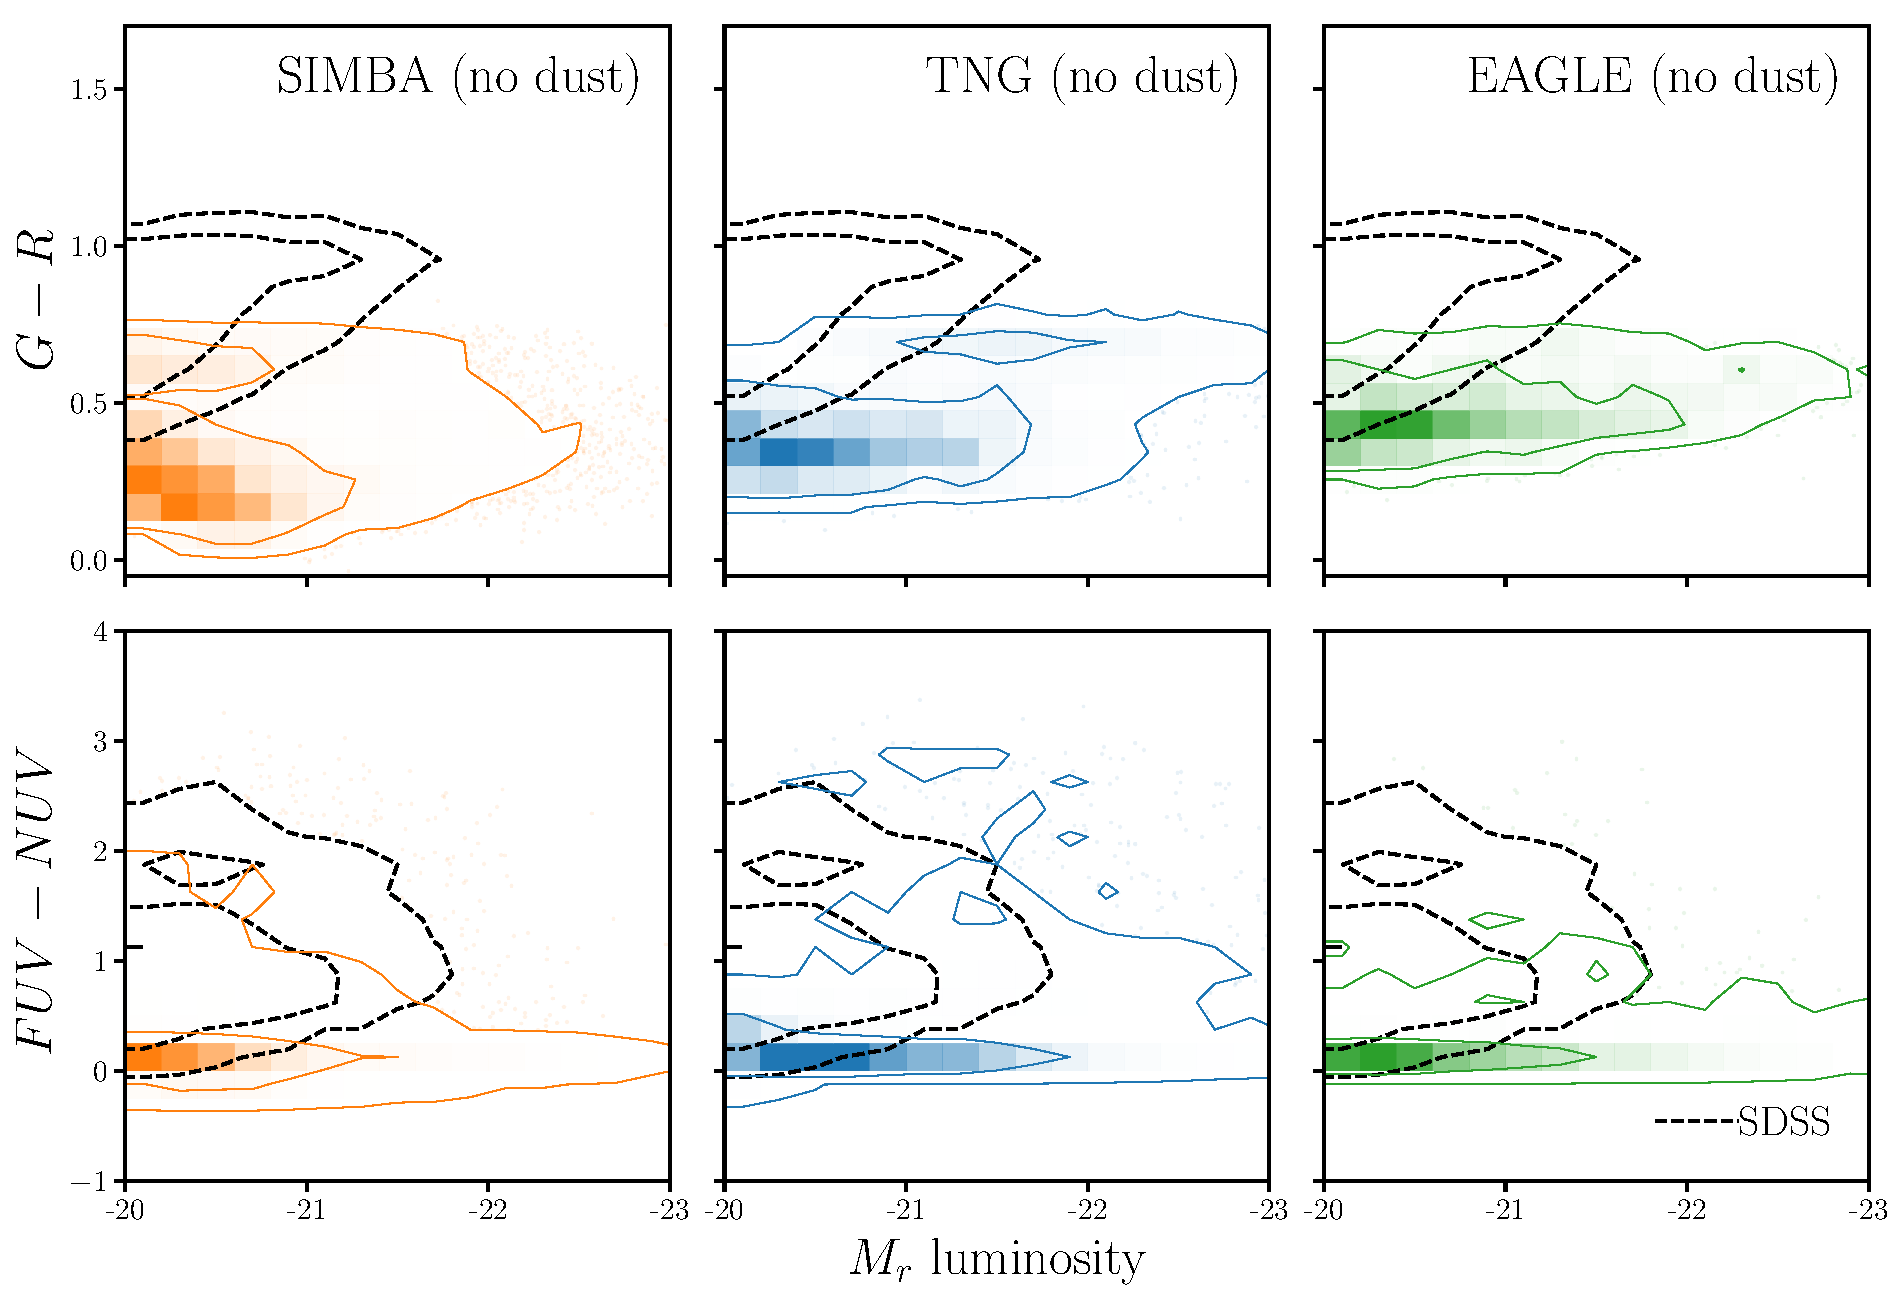
\includegraphics[width=0.9\textwidth]{figs/observables.pdf} 
    \caption{\label{fig:obs}
    \chedit{
        We present the forward modeled optical and UV color-magnitude relations
        of SIMBA (left), TNG (center), and EAGLE (right) galaxies
        \emph{assuming no dust attenuation}. We present $(\gr)-M_r$ in the top
        panels and $(\fnuv)-M_r$ in the bottom panels. The contours represent
        the 68 and 95\% of the distribution. We derive observables $M_r$, $\gr$, 
        and $\fnuv$ for the simulations using our forward model
        (Section~\ref{sec:fm}). For comparison, we include the color-magnitude
        relations of our SDSS sample (black dashed; Section~\ref{sec:obs}). 
        {\em Without dust attenuation, the hydrodynamical simulations do not
        reproduce the SDSS optical or UV color-magnitude relations.}
    }
    }
\end{center}
\end{figure}
